\documentclass[11pt]{article}
\usepackage[scaled=0.92]{helvet}
\usepackage{geometry}
\geometry{letterpaper,tmargin=1in,bmargin=1in,lmargin=1in,rmargin=1in}
\usepackage[parfill]{parskip} % Activate to begin paragraphs with an empty line rather than an indent %\usepackage{graphicx}
\usepackage{amsmath,amssymb, mathrsfs,  mathtools, dsfont}
\usepackage{tabularx}
\usepackage{tikz-cd}
\usepackage[font=footnotesize,labelfont=bf]{caption}
\usepackage{graphicx}
\usepackage{xcolor}
%\usepackage[linkbordercolor ={1 1 1} ]{hyperref}
%\usepackage[sf]{titlesec}
\usepackage{natbib}
\usepackage{../../Tianpei_Report}

%\usepackage{appendix}
%\usepackage{algorithm}
%\usepackage{algorithmic}

%\renewcommand{\algorithmicrequire}{\textbf{Input:}}
%\renewcommand{\algorithmicensure}{\textbf{Output:}}



\begin{document}
\title{Lecture 3: Tangent Vectors}
\author{ Tianpei Xie}
\date{Oct. 14th., 2022}
\maketitle
\tableofcontents
\newpage
\section{Tangent Vectors}
The central idea of calculus is \emph{\textbf{linear approximation}}. In order to make sense of calculus on manifolds, we need to introduce the \emph{tangent space} to a manifold at a point, which we can think of as a sort of "\emph{linear model}" for the manifold near the point. 
\subsection{Geometric Tangent Vectors}
\begin{itemize}
\item An element in Euclidean space $(x^1, \ldots, x^n) \in \bR^{n}$ has two distinct roles: 
\begin{enumerate}
\item As a \emph{\textbf{point}} in space, whose only property is its \emph{\textbf{location}} $(x^1, \ldots, x^n)$;
\item As a \emph{\textbf{vector}}, which are objects that have \emph{\textbf{magnitude}} and \emph{\textbf{direction}}, but whose location is irrelevant.

A vector $x = x^i e_i$ (where $e_i$ denotes the $i$-th standard basis vector) can be visualized as an arrow with its initial point \emph{anywhere} in $\bR^n$; what is relevant from the vector point of view is \emph{only which direction it points} and \emph{how long it is}.
\end{enumerate}

\begin{figure}
\begin{minipage}[t]{1\linewidth}
  \centering
  \centerline{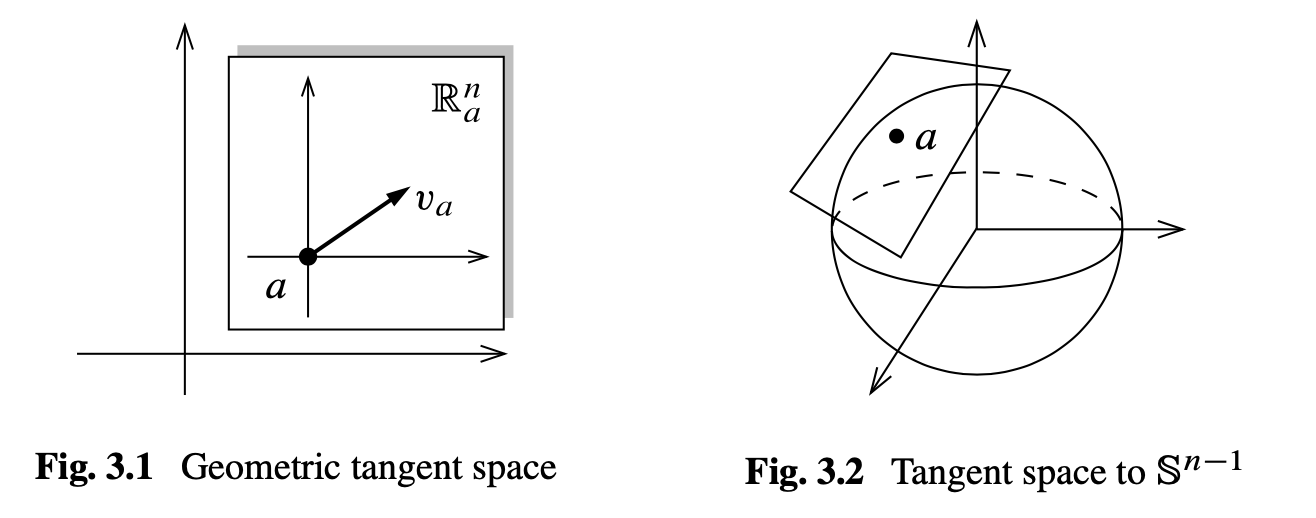
\includegraphics[scale = 0.6]{tangent_space_rn.png}}
\end{minipage}
\caption{\footnotesize{\textbf{A geometric tangent vector in $\bR^{n}$ (left); The tangent vector on $\bR^{n-1}.$ \citep{lee2003introduction}}}}
\label{fig: tangent_space_rn}
\end{figure}

\item \begin{definition}
Define the \underline{\emph{\textbf{geometric tangent space}}} to $\bR^n$ at $a$, denoted by $\bR_{a}^n$, to be the set $\set{a} \times \bR^n = \set{(a, v):  v \in \bR^n}$. A \emph{\textbf{geometric tangent vector}} in $\bR^n$ is an element of $\bR_{a}^n$ for some $a \in \bR^n$. 
\end{definition}
As a matter of notation, we abbreviate $(a, v)$ as $v_a$ (or sometimes $v|_a$ if it is clearer, for example if $v$ itself has a subscript).

\item We think of $v_a$ as the vector $v$ with its initial point at $a$ (Fig. \ref{fig: tangent_space_rn}).The set $\bR_{a}^n$ is a real \emph{vector space} under the natural operations
\begin{align*}
v_a + w_a = (v + w)_a, \quad c\,v_a = (c\,v)_a.
\end{align*} The vectors $e_i|_a$, $i = 1,\ldots,n$, are a basis for $\bR_{a}^n$. In fact, as a vector space, $\bR_{a}^n$ is essentially the same as $\bR^n$ itself.

\item \begin{definition}
If $a$ is a point of $\bR^n$, a map $w: \cC^{\infty}(\bR^n) \rightarrow \bR$ is called a \underline{\emph{\textbf{derivation at $a$}}} if it is \emph{\textbf{linear}} over $\bR$ and satisfies the following \emph{\textbf{product rule (Leibnitz rule)}}:
\begin{align}
w(f\,g) &= f(a)\,w(g) + g(a)\,w(f), \quad  \forall\,f,g \in \cC^{\infty}(\bR^{n})  \label{eqn: derivation_def}
\end{align}
\end{definition}

Let $T_{a}\bR^n$ denote the \emph{\textbf{set of all derivations}} of $\cC^{\infty}(\bR^n)$ at $a$. Clearly, $T_{a}\bR^n$  is a
\emph{vector space} under the operations
\begin{align*}
(w_1 + w_2)(f)  = w_1(f) + w_2(f), \quad (c\,w)(f) = c\,w(f).
\end{align*}

\item Note that by definition, a \emph{\textbf{derivation}} $w \in T_{a}\bR^n$ is a \emph{\textbf{linear functional}} on $\cC^{\infty}(\bR^n)$. Thus $T_{p}\bR^{n}$ is a functional space.

\item The most important (and perhaps somewhat surprising) fact about $T_{a}\bR^n$ is that it is \emph{\textbf{finite-dimensional}}, and in fact is naturally \emph{\textbf{isomorphic}} to the geometric tangent space $\bR_{a}^n$ that we defined above.

\item First, we have the following lemma
\begin{lemma} (\textbf{Properties of Derivations}).\\
Suppose $a \in \bR^n$, $w \in T_{a}\bR^n$, and $f, g \in \cC^{\infty}(\bR^n)$.
\begin{enumerate}
\item If $f$ is a constant function, then $w(f) = 0$. 
\item If $f(a) = g(a) = 0$, then $w(f\,g) = 0$.
\end{enumerate}
\end{lemma}

\item The next proposition shows that derivations at a are in \emph{one-to-one correspondence} with geometric tangent vectors.
\begin{proposition} \label{prop: iso_geo_tangent}
Let $a \in \bR^n$.
\begin{enumerate}
\item For each geometric tangent vector $v_a \in \bR_{a}^n$, the map $D_v|_a: \cC^{\infty}(\bR^n) \rightarrow \bR$ defined by following
\begin{align}
D_v|_a(f) &= D_{v}(f(a)) = \frac{d}{dt}\Big|_{t=0}f(a + t\,v). \label{eqn: directional_derivative}
\end{align}
 is a derivation at a.
\item The map $v_a \rightarrow D_v|_a$ is an \textbf{isomorphism} from $\bR_{a}^n$ onto $T_{a}\bR^n$.
\end{enumerate}
\end{proposition}
\begin{proof}
The fact that $D_v|_a$ is a derivation at $a$ is an immediate consequence of the product rule \eqref{eqn: derivation_def}.

To prove that the map $v_a \rightarrow D_v|_a$  is an isomorphism, we note first that it is \emph{linear}, as is easily checked. To see that it is \emph{injective}, suppose $v_a \in \bR_{a}^n$ has the property that $D_v|_a$ is the zero derivation. Writing $v_a = v^i e_i|_a$ in terms of the standard basis, and taking $f$ to be the $j$-th coordinate function $x^j: \bR^n \rightarrow \bR$, thought of as a smooth function on $\bR^n$, we obtain
\begin{align*}
 0 =D_v|_a(x^{j}) = v^{i}\partdiff{}{x^{i}}(x^{j})\Bigr|_{x = a} = v^{j}
\end{align*} where the last equality follows because $\partdiff{}{x^{i}}(x^{j}) = \delta_{i}(j)$. Since this is true for each $j$, it follows that $v_a$ is the zero vector. Note that 
\begin{align*}
D_v|_a(f) &= v^{i}\partdiff{f}{x^{i}}(a) = v^{i}\partdiff{}{x^{i}}(f)\Bigr|_{x = a}
\end{align*}

To prove surjectivity, let $w \in T_{a}\bR^n$ be arbitrary. Motivated by the computation in the preceding paragraph, we define $v_a = v^i e_i|_a$, where the real numbers $v^1, \ldots v^n$ are given by $v^i = w(x^i)$. We will show that $w = D_v|_a$.

To see this, let $f$ be any smooth real-valued function on $\bR^n$. By Taylor's theorem, we can write
\begin{align*}
f(x) &= f(a) + \sum_{i}\partdiff{f}{x^{i}}(a)(x^i - a^i) + \sum_{i,j}(x^i - a^i)(x^j - a^j)\int_{0}^{1}(1-t)\,\partdiff{^2 f}{x^{i}\partial x^{j}}(a + t(x - a))\,dt
\end{align*} Note that each term in the last sum above is a product of two smooth functions of $x$ that vanish at $x = a$. The derivation $w$ annihilates this entire sum by Lemma (b) above.

Thus
\begin{align*}
w(f) &= w(f(a)) + \sum_{i}w\paren{\partdiff{f}{x^{i}}(a)(x^i - a^i)}\\
&= 0 +  \sum_{i}\partdiff{f}{x^{i}}(a)(w(x^i) - w(a^i))\\
&= \sum_{i}\partdiff{f}{x^{i}}(a)v^{i} := D_v|_a(f). \qed
\end{align*}
\end{proof}

\item \begin{corollary}\label{coro: basis_tangent_space}
For any $a \in \bR^n$, the \textbf{$n$ derivations}
\begin{align}
\partdiff{}{x^{1}}\Bigr|_{a}, \ldots, \partdiff{}{x^{n}}\Bigr|_{a} \quad\text{defined by }\;\;\partdiff{}{x^{i}}\Bigr|_{a}(f) := \partdiff{f}{x^{i}}(a).
\end{align} form a \textbf{basis} for $T_{a}\bR^n$, which therefore has dimension $n$.
\end{corollary} Simply note that $\partdiff{}{x^{i}}\Bigr|_{a} = D_{e_i}|_a$.

\item The above proposition \emph{connects} two distinct concepts together via \emph{isomorphism}:
\begin{enumerate}
\item A \emph{\textbf{vector space}} $\bR_{a}^n$ at point $a$, which consists of all \emph{geometric tangent vectors} $v_a$. Each $v_a$ points to the \emph{direction} of tangent line at point $a$
\item A \emph{\textbf{functional space}} $T_{a}\bR^{n}$ associated with point $a$, which consists of all \emph{\textbf{derivations}} $w$. Each derivation $w = D_v\big|_{a}$ is a \emph{linear functional} that maps a smooth function on $\bR^{n}$ to its directional derivatives along vector $v$.
\end{enumerate}

\end{itemize}
\subsection{Tangent Vectors on Manifolds}
\begin{itemize}
\item 
\begin{definition}
Let $M$ be a smooth manifold with or without boundary, and let $p$ be a point of $M$. A \emph{\textbf{linear} map} $v: \cC^{\infty}(M) \rightarrow \bR$ is called a \underline{\textbf{\emph{derivation at p}}} if it satisfies the \emph{Leibnitz rule}:
\begin{align}
v(f\,g) &= f(a)\,v(g) + g(a)\,v(f), \quad \forall\,f,g \in \cC^{\infty}(M)  \label{eqn: derivation_def_man}
\end{align}

The set of all derivations of $\cC^{\infty}(M)$ at $p$, denoted by $T_{p}M$, is a \emph{vector space} called the \emph{\textbf{tangent space}} to $M$ at $p$. An element of $T_{p}M$ is called a \emph{\textbf{tangent vector}} at $p$.
\end{definition}

\item Similar to Euclidean space, the derivation on $M$ is a linear functional on smooth functions on $M$.

\item \begin{lemma} (\textbf{Properties of Tangent Vectors on Manifolds})\\
Suppose $M$ is a smooth manifold with or without boundary, $p \in M, v \in T_{p}M$, and $f, g \in \cC^{\infty}(M)$. 
\begin{enumerate}
\item If $f$ is a constant function, then $v(f) = 0$. 
\item If $f(p) = g(p) = 0$, then $v(f\,g) = 0$.
\end{enumerate}
\end{lemma}

\item With the motivation of geometric tangent vectors in $\bR^n$ in mind, you should visualize tangent vectors to $M$ as "arrows" that are tangent to $M$ and whose base points are attached to $M$ at the given point. Proofs of theorems about tangent vectors must, of course, be based on the abstract definition in terms of derivations, but your intuition should be guided as much as possible by the geometric picture.
\end{itemize}
\section{The Differential of a Smooth Map}
\begin{figure}
\begin{minipage}[t]{1\linewidth}
  \centering
  \centerline{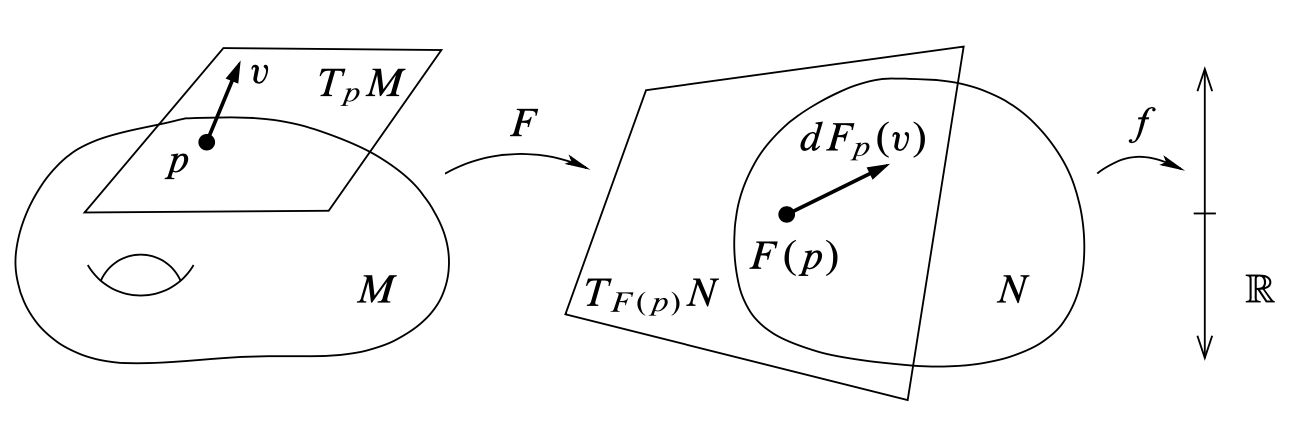
\includegraphics[scale = 0.6]{differentials.png}}
\end{minipage}
\caption{\footnotesize{\textbf{The differential \citep{lee2003introduction}}}}
\label{fig: differentials}
\end{figure}
\begin{itemize}
\item In the case of a smooth map between Euclidean spaces, the total derivative of the map at a point (represented by its Jacobian matrix) is a linear map that represents the ``\emph{best linear approximation}" to the map near the given point.

\item \begin{definition}
If $M$ and $N$ are \emph{smooth} manifolds with or without boundary and $F: M \rightarrow N$ is a \emph{smooth} map, for each $p \in M$ we define a map
\begin{align*}
dF_{p}: T_{p}M \rightarrow T_{F(p)}N ,
\end{align*} called the \underline{\emph{\textbf{differential}}} of $F$ at $p$ (Fig. \ref{fig: differentials}), as follows. Given $v \in T_{p}M$, we let $dF_{p}(v)$ be the \emph{\textbf{derivation} at $F(p)$} that \emph{\textbf{acts}} on $f \in \cC^{\infty}(N)$ by the rule 
\begin{align*}
dF_{p}(v)(f) &= v(f \circ F).
\end{align*} Note that if $f \in \cC^{\infty}(N)$, then $f \circ F \in \cC^{\infty}(M)$, so $v(f \circ F)$ makes sense. 
\end{definition}

\item The operator $dF_{p}(v): \cC^{\infty}(N) \rightarrow \bR$ is \emph{\textbf{linear}} because $v$ is, and is a \emph{\textbf{derivation}} at $F(p)$ because for any $f, g \in \cC^{\infty}(N)$ we have the product rule
\begin{align*}
dF_{p}(v)(fg) &= v((f\,g)\circ F) = v((f\circ F)\,(g \circ F))\\
&= (f\circ F)(p)\,v(g \circ F) + (g \circ F)(p)\,v(f \circ F)\\
&= f(F(p))\,dF_{p}(v)(g) + g(F(p))\,dF_{p}(v)(f)
\end{align*}

\item The \emph{differential} $dF_{p}$ is a \emph{\textbf{linear operator}} that maps a linear functional on $\cC^{\infty}(M)$ to another linear functional $\cC^{\infty}(N)$. This reflects the impact of smooth map $F: M \rightarrow N$.

\item \begin{proposition}\label{prop: diff_properties} (\textbf{Properties of Differentials}).\\
Let $M, N$, and $P$ be smooth manifolds with or without boundary, let $F: M \rightarrow N$ and $G: N \rightarrow P$ be smooth maps, and let $p \in M$.
\begin{enumerate}
\item $dF_{p}: T_{p}M \rightarrow T_{F(p)}N$ is \textbf{linear}.
\item $d(G \circ F)_{p} = dG_{F(p)} \circ dF_{p}: T_{p}M \rightarrow T_{(G \circ F)(p)}P$.
\item $d(\text{Id}_{M})_{p} = \text{Id}_{T_{p}M}: T_{p}M \rightarrow T_{p}M$.
\item If $F$ is a \textbf{diffeomorphism}, then $dF_{p}: T_{p}M \rightarrow T_{F(p)}N$ is an \textbf{isomorphism}, and
$(dF_{p})^{-1} = d(F^{-1})_{F(p)}$
\end{enumerate}
\end{proposition}

\item Our first important application of the differential will be to use \emph{coordinate charts} to relate the \emph{tangent space} to a point on a \emph{manifold} with the \emph{Euclidean tangent space}.

\item \begin{proposition} (\textbf{Tangent Vectors Act Locally})\\
Let $M$ be a smooth manifold with or without boundary, $p \in M$, and $v \in T_{p}M$. If $f, g \in \cC^{\infty}(M)$ agree on some neighborhood of $p$, then $v(f) = v(g)$.
\end{proposition}

\item \begin{proposition}\label{prop: tangent_open_subman} (\textbf{The Tangent Space to an Open Submanifold}). \\
Let $M $be a smooth manifold with or without boundary, let $U \subseteq M$ be an \textbf{open subset}, and let $\iota: U \xhookrightarrow{} M$ be the \textbf{inclusion map}. For every $p \in U$, the \textbf{differential} $d\iota_{p}: T_{p}U \rightarrow T_{p}M$ is an \textbf{isomorphism}.
\end{proposition}

Given an open subset $U \subseteq M$, the isomorphism $d\iota_{p}$ between $T_{p}U$ and $T_{p}M$ is \emph{canonically defined}, \emph{independently of any choices}. From now on we \emph{identify} $T_{p}U$ with $T_{p}M$ for any point $p \in U$. $d\iota_{p}(v)$ is the same derivation as $v$, thought of as acting on functions on the bigger manifold $M$ instead of functions on $U$. In particular, this means that any tangent vector $v \in T_{p}M$ can be \emph{unambiguously} applied to functions defined only in a \emph{neighborhood of $p$}, \emph{not necessarily on all of} $M$.

\item \begin{proposition} (\textbf{Dimension of the Tangent Space}).\\
If $M$ is an $n$-dimensional smooth manifold, then for each $p \in M$ the tangent space $T_{p}M$ is an $n$-dimensional vector space.
\end{proposition}
\begin{proof}
Given $p \in M$, let $(U, \varphi)$ be a smooth coordinate chart containing $p$. Because $\varphi$ is a diffeomorphism from $U$ onto an open subset $\widehat{U} \subseteq \bR^n$, it follows from property of differntials (Proposition \ref{prop: diff_properties} (d)) that $d\varphi_p$ is an \emph{isomorphism} from $T_{p}U$ to $T_{\varphi(p)}\widehat{U}$. Since Proposition \ref{prop: tangent_open_subman} guarantees that $T_{p}M \simeq T_{p}U$ and $T_{\varphi(p)}\widehat{U} \simeq T_{\varphi(p)}\bR^{n}$, it follows that $\text{dim}\, T_{p}M  = \text{dim}T_{\varphi(p)}\bR^{n} = n$. \qed
\end{proof}

\begin{figure}
\begin{minipage}[t]{1\linewidth}
  \centering
  \centerline{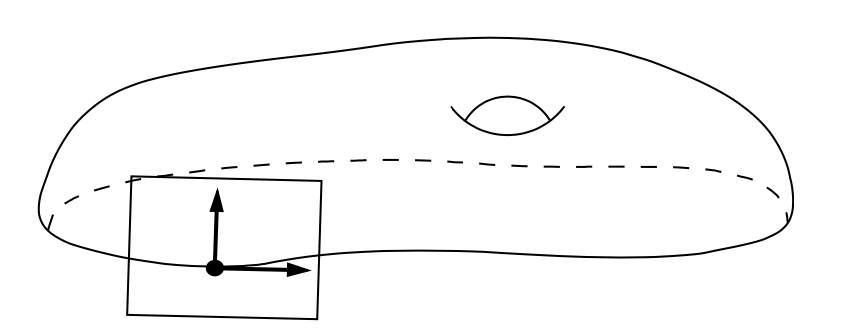
\includegraphics[scale = 0.6]{tangent_space_boundary.png}}
\end{minipage}
\caption{\footnotesize{\textbf{The tangent space on manifold with boundary \citep{lee2003introduction}}}}
\label{fig: tangent_space_boundary}
\end{figure}


\item Next we need to prove an analogous result for manifolds with boundary.
\begin{lemma}
Let $\iota: \bH^n \xhookrightarrow{} \bR^n$ denote the inclusion map. For any $a \in \partial\,\bH^n$, the differential $d\iota_a: T_{a}\bH^n \rightarrow T_{a}\bR^n$ is an isomorphism.
\end{lemma}

\begin{proposition} (\textbf{Dimension of Tangent Spaces on a Manifold with Boundary}) \citep{lee2003introduction}\\
Suppose $M$ is an $n$-dimensional smooth manifold \textbf{with boundary}. For each $p \in M$, $T_{p}M$ is an $n$-dimensional vector space.
\end{proposition}

\item Recall that every finite-dimensional vector space has a natural smooth manifold structure that is \emph{independent} of any choice of \emph{basis} or \emph{norm}. The following proposition shows that the \emph{\textbf{tangent space to a vector space} can be naturally identified with \textbf{the vector space itself}}.

\begin{proposition} (\textbf{The Tangent Space to a Vector Space}) \citep{lee2003introduction} \\
Suppose $V$ is a finite-dimensional vector space with its standard smooth manifold structure. For each point $a \in V$, the map $v \rightarrow D_v\big|_a$ defined by \eqref{eqn: directional_derivative} is a \textbf{canonical isomorphism} from $V$ to $T_{a}V$, such that for any linear map $L: V \rightarrow W$, the following diagram \textbf{commutes}:
\[
  \begin{tikzcd}
    V \arrow{r}{\simeq} \arrow[swap]{d}{L} & T_{a}V \arrow{d}{dL_{a}} \\
    W \arrow{r}{\simeq} & T_{L(a)}W
  \end{tikzcd}
\]
\end{proposition}

It is important to understand that each isomorphism $V \simeq T_a V$ is canonically defined, independently of any choice of basis (notwithstanding the fact that we used a choice of basis to prove that it is an isomorphism). Because of this result, we can routinely \emph{\textbf{identify}} tangent vectors to a finite-dimensional vector space with elements of the space itself.

\item There is another natural identification for tangent spaces to a product manifold.
\begin{proposition} (\textbf{The Tangent Space to a Product Manifold}) \citep{lee2003introduction} \\
 Let $M_1 ,\ldots, M_k$  be smooth manifolds, and for each $j$, let $\pi_j: M_1 \times \ldots \times M_k \rightarrow M_j$ be the projection on to the $M_j$ factor. For any point $p = (p_1, \ldots, p_k) \in M_1 \times \ldots \times M_k$, the map
\begin{align*}
\alpha: T_{p}(M_1 \times \ldots \times M_k) \rightarrow T_{p_1}M_1 \oplus \ldots \oplus T_{p_k}M_k
\end{align*} defined by
\begin{align}
\alpha(v) &= \paren{d(\pi_1)_p(v), \ldots, d(\pi_k)_p(v)} \label{eqn: diff_product_man}
\end{align} is an \textbf{isomorphism}. The same is true if one of the spaces $M_i$ is a smooth manifold with boundary.
\end{proposition} Once again, because the isomorphism \eqref{eqn: diff_product_man} is canonically defined, independently of any choice of coordinates, we can consider it as a canonical identification, and we will always do so. Thus, for example, we identify $T_{(p,q)}(M \times N)$ with $T_{p}M \oplus T_{q}N$, and treat $T_{p}M$ and $T_{q}N$ as \emph{\textbf{subspaces}} of $T_{(p,q)}(M \times N)$.
\end{itemize}


\section{Computations in Coordinates}
We will show how to do computations with tangent vectors and differentials in local coordinates.

\begin{figure}
\begin{minipage}[t]{1\linewidth}
  \centering
  \centerline{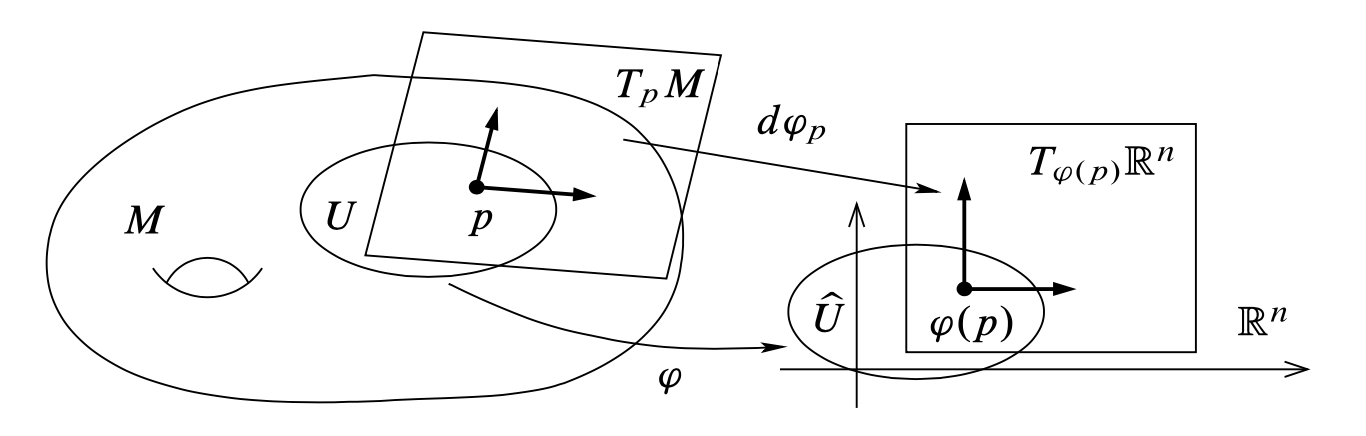
\includegraphics[scale = 0.6]{tangent_vec_coordinates.png}}
\end{minipage}
\caption{\footnotesize{\textbf{Tangent vectors in coordinates \citep{lee2003introduction}}}}
\label{fig: tangent_vec_coordinates}
\end{figure}

\subsection{The Derivation in Coordinates}
\begin{itemize}
\item First, suppose $M$ is a smooth manifold (without boundary), and let $(U, \varphi)$ be a smooth coordinate chart on $M$. Then $\varphi$ is, in particular, a \emph{\textbf{diffeomorphism}} from $U$ to an \emph{open subset} $\widehat{U} \subseteq \bR^n$. Combining Propositions \ref{prop: tangent_open_subman} and \ref{prop: diff_properties} (d), we see that $d\varphi_{p}: T_{p}M \rightarrow T_{\varphi(p)}\bR^n$ is an \emph{\textbf{isomorphism}}.

By Corollary \ref{coro: basis_tangent_space}, the derivations $\partdiff{}{x^{1}}\big|_{\varphi(p)}, \ldots, \partdiff{}{x^{n}}\big|_{\varphi(p)}$ form a basis for $T_{\varphi(p)}\bR^n$. Therefore, \emph{\textbf{the preimages of these vectors under the \emph{isomorphism} $d\varphi_p$ form a basis for $T_{p}M$}} (Fig. \ref{fig: tangent_vec_coordinates}).

In keeping with our standard practice of treating coordinate maps as \emph{identifications} whenever possible, we use the notation $\partdiff{}{x^{i}}\big|_{p}$ for these vectors, characterized by either of the \textbf{following expressions}:
\begin{align}
\partdiff{}{x^{i}}\Bigr|_{p} &:= (d\varphi_{p})^{-1}\paren{\partdiff{}{x^{i}}\Bigr|_{\varphi(p)}} 
= d(\varphi^{-1})_{\varphi(p)}\paren{\partdiff{}{x^{i}}\Bigr|_{\varphi(p)}} \label{eqn: identification_tangent_basis}
\end{align}

\item Unwinding the definitions, we see that $\partdiff{}{x^{i}}\big|_{p}$ acts on a function $f \in \cC^{\infty}(U)$ by
\begin{align*}
\partdiff{}{x^{i}}\Bigr|_{p}(f) &= \partdiff{}{x^{i}}\Bigr|_{\varphi(p)}(f \circ \varphi^{-1}) = \partdiff{\widehat{f}}{x^{i}}(\widehat{p})
\end{align*} where $\widehat{f} = f \circ \varphi^{-1}$ is the \emph{coordinate representation} of $f$, and $\widehat{p} = (p^1, \ldots, p^n) = \varphi(p)$ is the \emph{coordinate representation} of $p$.

\begin{definition}
In other words, $\partdiff{}{x^{i}}\big|_{p}$ is just the \textbf{\emph{derivation}} that takes the \emph{$i$-th partial derivative of (the coordinate representation of) $f$ at (the coordinate representation of) $p$}. The vectors $\partdiff{}{x^{i}}\big|_{p}$ are called the \underline{\emph{\textbf{coordinate vectors at p} associated with the given coordinate system}}.
\end{definition}

In the special case of standard coordinates on $\bR^n$, the vectors $\partdiff{}{x^{i}}\big|_{p}$ are literally the partial derivative operators.

\item When $M$ is a \emph{smooth manifold \textbf{with boundary}} and $p$ is an interior point, the discussion above applies verbatim. For $p \in \partial\,M$, the only change that needs to be made is to substitute $\bH^n$ for $\bR^n$, with the understanding that the notation $\partdiff{}{x^{i}}\big|_{\varphi(p)}$ can be used interchangeably to denote either an element of $T_{\varphi(p)}\bR^n$ or an element of $T_{\varphi(p)}\bH^n$, in keeping with our convention of considering the isomorphism $d\iota_{\varphi(p)}: T_{\varphi(p)}\bH^n \rightarrow T_{\varphi(p)}\bR^n$ as an \emph{identification}. The $n$-th coordinate vector $\partdiff{}{x^{n}}\big|_{p}$ should be interpreted as a \emph{\textbf{one-sided derivative}} in this case.

\item We summarize our discussion as below proposition.
\begin{proposition}
Let $M$ be a smooth $n$-manifold with or without boundary, and let $p \in M$. Then $T_{p}M$ is an $n$-dimensional vector space, and for any smooth chart $(U, \varphi)$ containing $p$, the \textbf{coordinate vectors} $\partdiff{}{x^{1}}\big|_{p}, \ldots, \partdiff{}{x^{n}}\big|_{p}$ \textbf{form a basis} for $T_{p}M$.
\end{proposition}

\item 
\begin{definition}
A tangent vector $v \in T_{p}M$ can be written \textbf{\emph{uniquely}} as a linear combination
\begin{align}
v&=v^{i} \partdiff{}{x^{i}}\Bigr|_{p} \label{eqn: tangent_vec_decomp}
\end{align} where we use the \emph{Einstein summation convention} as usual. 

The \emph{ordered basis} $(\partdiff{}{x^{i}}\big|_{p})$ is called a \emph{\textbf{coordinate basis}} for $T_{p}M$, and the numbers $(v^1, \ldots, v^n)$ are called the \emph{\textbf{components}} of $v$ \emph{with respect to the coordinate basis}.
\end{definition}

\item If $v$ is known, its components can be computed easily from its action on the coordinate functions. For each $j$, the components of $v$ are given by $v^j = v(x^{j})$ (where we think of $x^j$ as a smooth real-valued function on $U$), because
\begin{align*}
v(x^{j}) &= v^{i} \partdiff{}{x^{i}}\Bigr|_{p}(x^{j}) = v^{i} \partdiff{x^{j}}{x^{i}}(p) = v^{i}\delta_{i}^{j} = v_{j}
\end{align*}
\end{itemize}

\subsection{The Differential in Coordinates}
\begin{itemize}
\item Next we explore how differentials look in coordinates. We begin by considering the special case of a smooth map $F: U \rightarrow V$, where $U \subseteq \bR^n$ and $V \subseteq \bR^m$ are open subsets of \emph{Euclidean spaces}.  For any $p \in U$ , we will determine the matrix of $dF_p: T_{p}\bR^n \rightarrow T_{F(p)}\bR^m$ in terms of the standard coordinate bases.

Using $(x^1,\ldots, x^n)$ to denote the coordinates in the domain and $(y^1,\ldots, y^m)$ to denote those in the codomain, we use the \emph{\textbf{chain rule}} to compute the action of $dF_p$ on a typical basis vector as follows:
\begin{align*}
dF_p\paren{\partdiff{}{x^{i}}\Bigr|_{p}}(f) &= \partdiff{}{x^{i}}\Bigr|_{p} (f \circ F) \\
&= \partdiff{f}{y^{j}}(F(p)) \partdiff{F^{j}}{x^{i}}(p) \\
&= \paren{\partdiff{F^{j}}{x^{i}}(p)\,\partdiff{}{y^{j}}\Bigr|_{F(p)}}(f) 
\end{align*}

\begin{figure}
\begin{minipage}[t]{1\linewidth}
  \centering
  \centerline{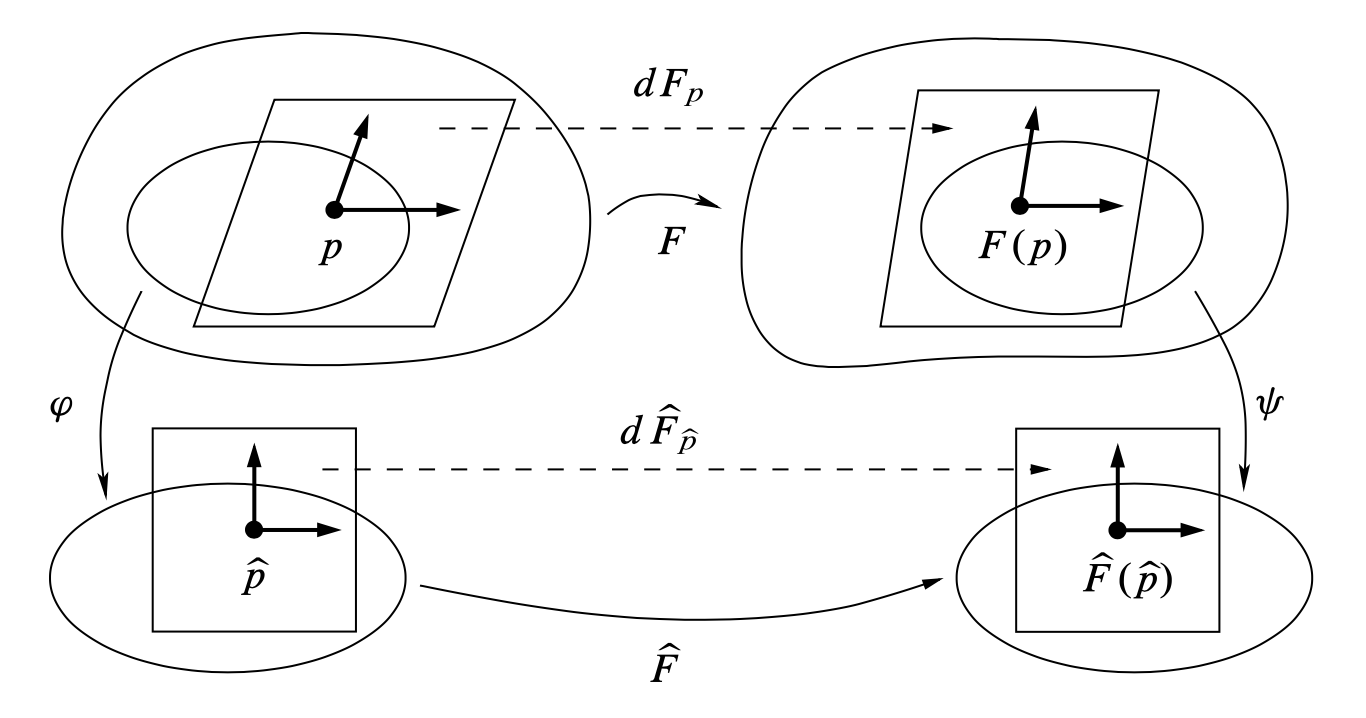
\includegraphics[scale = 0.5]{differential_coordinate.png}}
\end{minipage}
\caption{\footnotesize{\textbf{The differential in coordinates \citep{lee2003introduction}}}}
\label{fig: differential_coordinate}
\end{figure}

\item \begin{definition}
The action of \emph{\textbf{differential}} of $F: U \rightarrow V$ , where $U \subseteq \bR^n$ and $V \subseteq \bR^m$ \emph{on a typical basis vector} can be represented as
\begin{align}
dF_p\paren{\partdiff{}{x^{i}}\Bigr|_{p}} &= \partdiff{F^{j}}{x^{i}}(p)\,\partdiff{}{y^{j}}\Bigr|_{F(p)} \label{eqn: differential_coordinate}
\end{align} where $(x^1,\ldots, x^n)$ is the coordinates of $U$ and $(y^1,\ldots, y^m)$ is the coordinate of $V$.
\end{definition} 

\item In other words, the \emph{\textbf{matrix}} of $dF_p$ in terms of the coordinate bases is 
\begin{align}
\brac{\begin{array}{ccc}
\dfrac{\partial\,F^{1}}{\partial\,x^{1}}(p)& \ldots& \dfrac{\partial\,F^{1}}{\partial\,x^{n}}(p)\\
\vdots & \ddots & \vdots\\
\dfrac{\partial\,F^{m}}{\partial\,x^{1}}(p)& \ldots& \dfrac{\partial\,F^{m}}{\partial\,x^{n}}(p)
\end{array}}_{m \times n}  \label{eqn: differential_coordinate_mat}
\end{align} This matrix is none other than \emph{\textbf{the Jacobian matrix}} of $F$ at $p$, which is the \emph{matrix representation} of the \emph{\textbf{total derivative}} $DF_{p}: \bR^n \rightarrow \bR^m$. 
Therefore, in this case, $dF_p: T_{p}\bR^n \rightarrow T_{F(p)}\bR^m$ corresponds to \emph{the total derivative} $DF_{p}: \bR^n \rightarrow \bR^m$, under our usual identification of Euclidean spaces with their tangent spaces. The same calculation applies if $U$ is an open subset of $\bH^n$ and $V$ is an open subset of $\bH^m$.

\item Now consider the more general case of a smooth map $F: M \rightarrow N$ between smooth manifolds with or without boundary.   Choosing smooth coordinate charts $(U,\varphi)$ for $M$ containing $p$ and $(V, \psi)$  for $N$ containing $F(p)$, we obtain the \emph{\textbf{coordinate representation}} $\widehat{F} = \psi \circ F \circ \varphi^{-1}: \varphi(U \cap F^{-1}(V)) \rightarrow \psi(V)$ (Fig \ref{fig: differential_coordinate}). Let $\widehat{p} = \varphi(p)$ be \emph{coordinate representation} of $p$.

By the computation above, $d\widehat{F}_{\widehat{p}}$ is represented with respect to the standard coordinate bases by the Jacobian matrix of $\widehat{F}$ at $\widehat{p}$. Using the fact that $\psi^{-1} \circ \widehat{F} =  F \circ \varphi^{-1}$, we compute
\begin{align*}
dF_{p}\paren{\partdiff{}{x^{i}}\Bigr|_{p}} &= dF_{p}\paren{d (\varphi^{-1})_{\widehat{p}}\paren{\partdiff{}{x^{i}}\Bigr|_{\widehat{p}}}} \\
&= d(\psi^{-1})_{\widehat{F}(\widehat{p})}\paren{d\widehat{F}_{\widehat{p}}\paren{\partdiff{}{x^{i}}\Bigr|_{\widehat{p}}} }\\
&= d(\psi^{-1})_{\widehat{F}(\widehat{p})}\paren{ \partdiff{\widehat{F}^{j}}{x^{i}}(\widehat{p})\,\partdiff{}{y^{j}}\Bigr|_{\widehat{F}(\widehat{p})} }\\
&= \partdiff{\widehat{F}^{j}}{x^{i}}(\widehat{p})\,\paren{d(\psi^{-1})_{\widehat{F}(\widehat{p})}\partdiff{}{y^{j}}\Bigr|_{\widehat{F}(\widehat{p})}}\\
&= \partdiff{\widehat{F}^{j}}{x^{i}}(\widehat{p})\,\partdiff{}{y^{j}}\Bigr|_{p}
\end{align*}

\begin{definition}
For a smooth map $F: M \rightarrow N$ between smooth manifolds with or without boundary, the action of \emph{\textbf{differential}} $dF_{p}$ on a typical basis vector can be represented as
\begin{align}
dF_{p}\paren{\partdiff{}{x^{i}}\Bigr|_{p}} &= \partdiff{\widehat{F}^{j}}{x^{i}}(\widehat{p})\,\partdiff{}{y^{j}}\Bigr|_{F(p)}, \label{eqn: differential_coordinate_manifold}
\end{align} where  $\widehat{F} = \psi \circ F \circ \varphi^{-1}: \varphi(U \cap F^{-1}(V)) \rightarrow \psi(V)$ is the coordinate representation of $F$ under smooth charts $(U,\varphi)$ for $M$ and $(V, \psi)$ for $N$. Also $\widehat{p} = \varphi(p)$  is the coordinate representation of $p$. The matrix for $[\partdiff{\widehat{F}^{j}}{x^{i}}(\widehat{p})]_{j,i}$ is the Jacobian matrix.

That is $dF_{p}$ is represented in coordinate bases by the \emph{\textbf{Jacobian matrix}} of (the coordinate representative of) $F$.
\end{definition}

\item In fact, the definition of the \emph{differential} was cooked up precisely to give a \emph{\textbf{coordinate-independent}} meaning to \emph{the Jacobian matrix}.

\item \begin{definition}
In the differential geometry literature, the \emph{differential} is sometimes called the \emph{\textbf{tangent map}}, \emph{\textbf{the total derivative}}, or simply the derivative of $F$. Because it "\emph{\textbf{pushes}}" \emph{tangent vectors} \emph{\textbf{forward}} from the domain manifold to the codomain, it is also called \emph{\textbf{the (pointwise) \underline{pushforward}}}. Different authors denote it by symbols such as
\begin{align*}
F'(p), \quad D\,F(p), \quad D\,F, \quad F^{*},\quad T\,F, \quad T_{p}F.
\end{align*}

\end{definition}
\end{itemize}

\subsection{Change of Coordinates}
\begin{itemize}
\item Suppose $(U, \varphi)$ and $(V, \psi)$ are two smooth charts on $M$, and $p \in U \cap V$. Let us denote the coordinate functions of $\varphi$ by $(x^i)$ and those of $\psi$ by $(\widetilde{x}^i)$. Any tangent vector at $p$ can be represented with respect to either basis $(\partdiff{}{x^{i}}\big|_{p})$ or $(\partdiff{}{\widetilde{x}^{i}}\big|_{p})$. 


\begin{figure}
\begin{minipage}[t]{1\linewidth}
  \centering
  \centerline{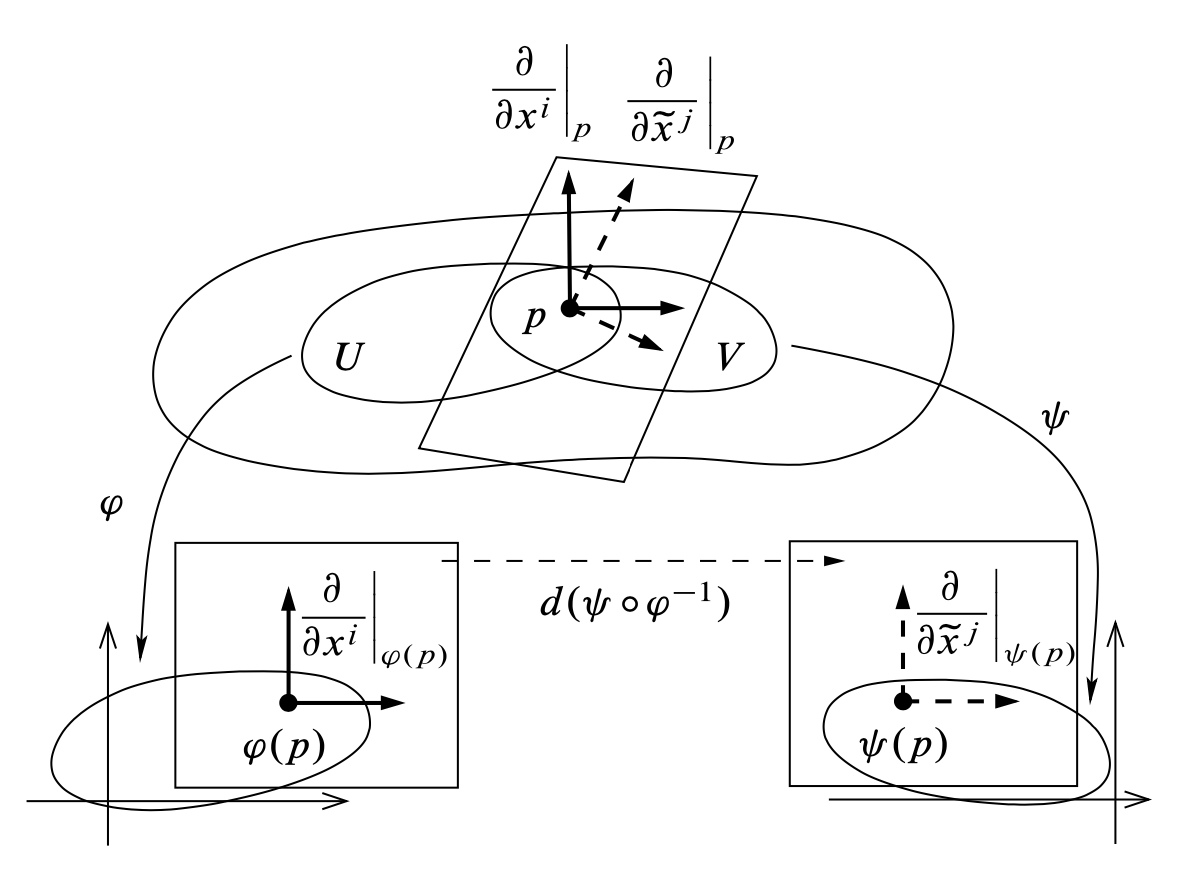
\includegraphics[scale = 0.5]{change_of_coordinates.png}}
\end{minipage}
\caption{\footnotesize{\textbf{The change of coordinates \citep{lee2003introduction}}}}
\label{fig: change_of_coordinates}
\end{figure}

To \emph{\textbf{change of coordinates}}, we write the transition map $\psi \circ \varphi^{-1}: \varphi(U \cap V) \rightarrow \psi(U \cap V)$ in the following shorthand notation:
\begin{align*}
\psi \circ \varphi^{-1}(x) &= (\widetilde{x}^{1}(x), \ldots, \widetilde{x}^{n}(x)).
\end{align*}
Here we are indulging in a typical abuse of notation: in the expression $\widetilde{x}^{i}(x)$, we
think of $\widetilde{x}^{i}(x)$ as a \emph{\textbf{coordinate function}} (whose domain is an open subset of $M$; identified with an open subset of $\bR^n$ or $\bH^n$); but we think of $x$ as representing a \emph{\textbf{point}} (in this case, in $\varphi(U \cap V)$ ). By \eqref{eqn: differential_coordinate_manifold}, the differential $d(\psi \circ \varphi^{-1})_{\varphi(p)}$ can be written 
\begin{align*}
d(\psi \circ \varphi^{-1})_{\varphi(p)}\paren{\partdiff{}{x^{i}}\Bigr|_{\varphi(p)}}
&=\partdiff{\widetilde{x}^{j}}{x^{i}}(\varphi(p))\,\partdiff{}{\widetilde{x}^{j}}\Bigr|_{\psi(p)}.
\end{align*} See Fig \ref{fig: change_of_coordinates}.  Using the definition of coordinate vectors, we obtain 
\begin{align*}
\partdiff{}{x^{i}}\Bigr|_{p} &= d(\varphi^{-1})_{\varphi(p)}\paren{\partdiff{}{x^{i}}\Bigr|_{\varphi(p)}} \\
&= d(\psi^{-1})_{\psi(p)}\circ d(\psi \circ \varphi^{-1})_{\varphi(p)}\paren{\partdiff{}{x^{i}}\Bigr|_{\varphi(p)}} \\
&= d(\psi^{-1})_{\psi(p)}\paren{\partdiff{\widetilde{x}^{j}}{x^{i}}(\varphi(p))\,\partdiff{}{\widetilde{x}^{j}}\Bigr|_{\psi(p)}} \\
&=\partdiff{\widetilde{x}^{j}}{x^{i}}(\varphi(p))\,d(\psi^{-1})_{\psi(p)}\paren{\partdiff{}{\widetilde{x}^{j}}\Bigr|_{\psi(p)}} \\
&= \partdiff{\widetilde{x}^{j}}{x^{i}}(\widehat{p})\,\partdiff{}{\widetilde{x}^{j}}\Bigr|_{p} 
\end{align*} where again we have written $\widehat{p} = \varphi(p)$. 

\item \begin{remark}
Given two smooth charts $(U, \varphi)$ and $(V, \psi)$ on $M$, the \emph{\textbf{change of coordinates}} between basis vectors $(\partdiff{}{x^{i}}\big|_{p})$ (of $\varphi$) and $(\partdiff{}{\widetilde{x}^{i}}\big|_{p})$ (of $\psi$) is obtained via
\begin{align}
\partdiff{}{x^{i}}\Bigr|_{p} &=  \partdiff{\widetilde{x}^{j}}{x^{i}}(\widehat{p})\,\partdiff{}{\widetilde{x}^{j}}\Bigr|_{p}   \label{eqn: change_of_coordinates}
\end{align} where $\widehat{p} = \varphi(p)$ is the coordinate representation of $p$ under $\varphi$. 
\end{remark}
This formula is easy to remember, because it looks exactly the same as the \emph{chain rule} for partial derivatives in $\bR^n$.

Applying this to the components of a vector $v = v^i \partdiff{}{x^{i}}\big|_{p} = \widetilde{v}^j \,\partdiff{}{\widetilde{x}^{i}}\big|_{p}$, we find that the components of $v$ transform by the rule
\begin{align}
\widetilde{v}^{j} &= \partdiff{\widetilde{x}^{j}}{x^{i}}(\widehat{p})\,v^i   \label{eqn: change_of_coordinates_full}
\end{align}

\item
\begin{example}
The transition map between polar coordinates and standard coordinates in suitable open subsets of the plane is given by 
\begin{align*}
x &=  r\,\cos(\theta) \\
y &=  r\,\sin(\theta) 
\end{align*} Let $p$ be the point in $\bR^2$ whose polar coordinate representation is $(r, \theta) = (2, \pi/2)$, and let $v \in T_{p} \bR^2$ be the tangent vector whose polar coordinate representation is
\begin{align*}
v &= 3\partdiff{}{r}\Bigr|_{p} - \partdiff{}{\theta}\Bigr|_{p}.
\end{align*}

Applying \eqref{eqn: change_of_coordinates} to the coordinate vectors, we find
\begin{align*}
\partdiff{}{r}\Bigr|_{p} &= \partdiff{x(2, \pi/2)}{r}\partdiff{}{x}\Bigr|_{p} + \partdiff{y(2, \pi/2)}{r}\partdiff{}{y}\Bigr|_{p} \\
&= \cos\paren{\frac{\pi}{2}}\partdiff{}{x}\Bigr|_{p} + \sin\paren{\frac{\pi}{2}}\partdiff{}{y}\Bigr|_{p} = \partdiff{}{y}\Bigr|_{p} \\
\partdiff{}{\theta}\Bigr|_{p} &= \partdiff{x(2, \pi/2)}{\theta}\partdiff{}{x}\Bigr|_{p} + \partdiff{y(2, \pi/2)}{\theta}\partdiff{}{y}\Bigr|_{p} \\
&= -2\,\sin\paren{\frac{\pi}{2}}\partdiff{}{x}\Bigr|_{p}  + 2\,\cos\paren{\frac{\pi}{2}}\partdiff{}{y}\Bigr|_{p}
=-2\,\partdiff{}{x}\Bigr|_{p} 
\end{align*} and thus $v$ has the following coordinate representation in standard coordinates:
\begin{align*}
v &= 3\partdiff{}{y}\Bigr|_{p} + 2\,\partdiff{}{x}\Bigr|_{p}.
\end{align*}
\end{example}

\item \emph{\textbf{One important fact}} to bear in mind is that \textbf{\emph{each coordinate vector} $\partial /\partial\,x^i\big|_{p}$ depends on \emph{the entire coordinate system}}, not just on the single coordinate function $x^i$. 

Geometrically, this reflects the fact that $\partial /\partial\,x^i\big|_{p}$ is the \emph{\textbf{derivation}} obtained by differentiating with respect to $x^i$ while \emph{all the other coordinates} are held \emph{constant}. If the coordinate functions other than $x^i$ \emph{are changed}, then the \emph{direction} of this \emph{coordinate derivative can change}.
\end{itemize}

\section{The Tangent Bundle}
\begin{itemize}
\item Often it is useful to consider the set of \emph{all tangent vectors at all points} of a manifold. 
\begin{definition}
Given a smooth manifold $M$ with or without boundary, the \underline{\emph{\textbf{tangent bundle}}} of $M$, denoted by $TM$, is defined as the \emph{\textbf{disjoint union}} of \emph{the tangent spaces} \emph{\textbf{at all points}} of $M$:
\begin{align*}
TM &= \bigsqcup_{p \in M}T_{p}M.
\end{align*}
\end{definition}

\item We usually write an \emph{\textbf{element}} of this disjoint union as \emph{\textbf{an ordered pair}} $(p, v)$, with $p \in M$ and $v \in T_{p}M$.

\item \begin{definition}
The tangent bundle comes equipped with a \emph{\textbf{natural projection map}} $\pi: TM \rightarrow M$, which sends each vector in $T_{p}M$ to the point $p$ at which it is tangent: $\pi(p, v) = p$.
\end{definition}

We will often commit the usual mild sin of identifying $T_{p}M$ with its image under the canonical injection $v \mapsto (p, v)$, and will use any of the notations $(v, p),  v_{p}$ and $v$ for a tangent vector in $T_{p}M$, depending on how much emphasis we wish to give to the point $p$.

\begin{figure}
\begin{minipage}[t]{1\linewidth}
  \centering
  \centerline{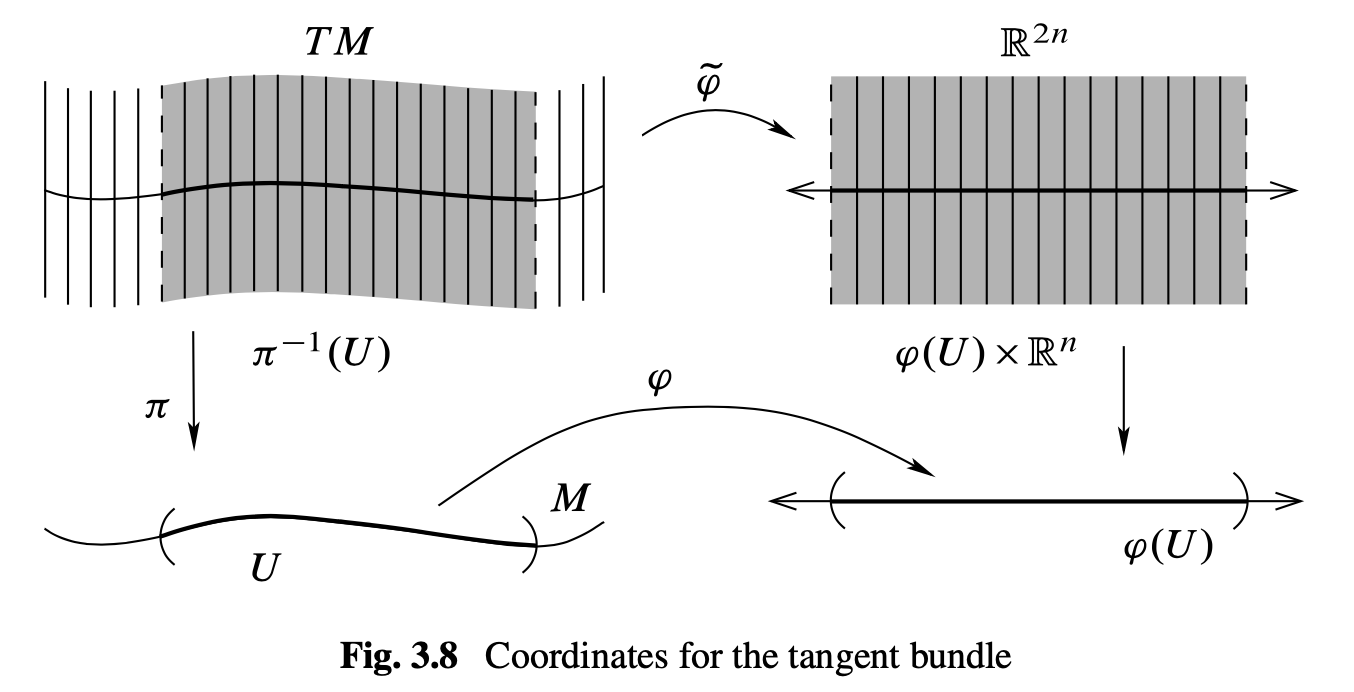
\includegraphics[scale = 0.5]{coordinate_tangent_bundle.png}}
\end{minipage}
\caption{\footnotesize{\textbf{Coordinates for the tangent bundle \citep{lee2003introduction}}}}
\label{fig: coordinate_tangent_bundle}
\end{figure}

\item \begin{example}
In the special case $M = \bR^n$, using Proposition \ref{prop: iso_geo_tangent}, we see that the tangent bundle of $\bR^n$ can be canonically identified with the union of its geometric tangent spaces, which in turn is just the Cartesian product of $\bR^n$ with itself:
\begin{align*}
T\bR^{n} = \bigsqcup_{p \in M}T_{p}\bR^{n} \simeq \bigsqcup_{p \in M}\bR_{p}^{n} = \bigsqcup_{p \in M}\set{p}\times \bR^{n} = \bR^{n} \times \bR^{n}.
\end{align*} An element $(a, v)$ of this Cartesian product can be thought of as representing \emph{either the geometric tangent vector} $v_a$ or the \emph{derivation} $D_v\big|_{a}$ defined by \eqref{eqn: directional_derivative}. 

Be warned, however, that \textbf{in general} the tangent bundle of a smooth manifold \textbf{cannot} be identified in any natural way with a Cartesian product, because \emph{there is no canonical way to identify tangent spaces at different points with each other}.
\end{example}

\item 
\begin{proposition} (\textbf{Tangent Bundle Is a Manifold}) \citep{lee2003introduction}\\
For any smooth n-manifold $M$, the tangent bundle $TM$ has a \textbf{natural topology} and \textbf{smooth structure} that make it into a \underline{\textbf{$2n$-dimensional smooth manifold}}. With respect to this structure, the projection $\pi: TM \rightarrow M$ is \textbf{smooth}.
\end{proposition}
\begin{proof}
We begin by defining the maps that will become our smooth charts. Given any smooth chart $(U, \varphi)$ for $M$, note that $\pi^{-1}(U) \subseteq TM$ is the set of \emph{all tangent vectors} to $M$ at all points of $U$. Let $(x^1, \ldots, x^n)$ denote the coordinate functions of $\varphi$, and define a map $\widetilde{\varphi}: \pi^{-1}(U) \rightarrow \bR^{2n}$ by
\begin{align}
\widetilde{\varphi}\paren{v^{i}\partdiff{}{x^{i}}\Bigr|_{p}} &= (x^{1}(p), \ldots, x^{n}(p), v^{1}, \ldots, v^{n}). \label{eqn: tangent_bundle_coordinate_chart}
\end{align} (See Fig \ref{fig: coordinate_tangent_bundle}.) Its image set is $\varphi(U) \times \bR^n$, which is an open subset of $\bR^{2n}$. It is a \emph{bijection} onto its image, because its \emph{inverse} can be written explicitly as
\begin{align*}
\widetilde{\varphi}^{-1}(x^{1}, \ldots, x^{n}, v^{1}, \ldots, v^{n}) &= v^{i}\partdiff{}{x^{i}}\Bigr|_{\varphi^{-1}(x)}.
\end{align*}

Now suppose we are given two smooth charts $(U, \varphi)$ and $(V, \psi)$ for $M$ and let $(\pi^{-1}(U), \widetilde{\varphi})$ and $(\pi^{-1}(V), \widetilde{\psi})$ be corresponding charts in $TM$. The sets
\begin{align*}
\widetilde{\varphi}\paren{\pi^{-1}(U) \cap \pi^{-1}(V)} &= \varphi(U\cap V) \times \bR^{n}\\
\widetilde{\psi}\paren{\pi^{-1}(U) \cap \pi^{-1}(V)} &= \psi(U\cap V) \times \bR^{n}
\end{align*} are open in $\bR^{2n}$, and the transition map $\widetilde{\psi} \circ \widetilde{\varphi}^{-1}: \varphi(U\cap V) \times \bR^{n} \rightarrow  \psi(U\cap V) \times \bR^{n}$ can be written explicitly using the change of coordinate equation  \eqref{eqn: change_of_coordinates_full}
\begin{align*}
\widetilde{\psi} \circ \widetilde{\varphi}^{-1}(x^{1}, \ldots, x^{n}, v^{1}, \ldots, v^{n})
&= \paren{\widetilde{x}^{1}, \ldots, \widetilde{x}^{n}, \partdiff{\widetilde{x}^{1}}{x^{j}}\,v^j, \ldots, \partdiff{\widetilde{x}^{n}}{x^{j}}\,v^j   }.
\end{align*} This is clearly \emph{smooth}.

Choosing a countable cover $\set{U_i}$ of $M$ by smooth coordinate domains, we obtain a countable cover of $TM$ by coordinate domains  $\set{\pi^{-1}(U)}$ satisfying conditions (1)-(4) of the smooth manifold chart lemma. (See lecture 1.) To check the \emph{Hausdorff condition} (5), just note that any two points in the same \emph{fiber} of $\pi$ lie in one chart, while if $(p, v)$ and $(q, w)$ lie in different fibers, there exist \emph{disjoint} smooth coordinate domains $U$, $V$ for $M$ such that $p \in U$ and $q \in V$, and then $\pi^{-1}(U)$ and $\pi^{-1}(V)$ are \emph{disjoint coordinate neighborhoods} containing $(p, v)$ and $(q, w)$, respectively.

To see that $\pi$ is smooth, note that with respect to charts $(U, \varphi)$ for $M$ and $(\pi^{-1}(U), \widetilde{\varphi})$ for $TM$, its coordinate representation is $\pi(x, v) = x$.\qed
\end{proof}

\item \begin{definition}
The coordinates $(x^i, v^i)$ given by 
\begin{align*}
\widetilde{\varphi}\paren{v^{i}\partdiff{}{x^{i}}\Bigr|_{p}} &= (x^{1}(p), \ldots, x^{n}(p), v^{1}, \ldots, v^{n}). 
\end{align*}  are called \emph{\textbf{natural coordinates}} on $TM$.
\end{definition}

\item \begin{proposition}
If $M$ is a smooth $n$-manifold with or without boundary, and $M$ can be covered by \textbf{a single smooth chart}, then $TM$ is diffeomorphic to $M \times \bR^n$.
\end{proposition}

\item \begin{remark}
Although the picture of a product $U \times \bR^n$ is a useful way to visualize the smooth structure on a tangent bundle locally as in Fig. \ref{fig: coordinate_tangent_bundle} do \textbf{not} be misled into imagining that every tangent bundle is \emph{\emph{globally diffeomorphic}} (or even \emph{\textbf{homeomorphic}}) to a \emph{product of the manifold with $\bR^n$}. \textbf{This is not the case for most smooth manifolds}.
\end{remark}

\item \begin{definition}
By putting together the \emph{\textbf{differentials}} of $F$ \emph{\textbf{at all points}} of $M$, we obtain a \emph{\textbf{globally} defined map} between \emph{tangent bundles}, called \underline{\emph{\textbf{the global differential}}} or \emph{\textbf{global tangent map}} and denoted by $dF: TM \rightarrow TN$.

This is just the map whose restriction to each tangent space $T_{p}M \subseteq TM$ is $dF_{p}$.
\end{definition}

When we apply the differential of $F$ to a specific vector $v \in T_{p}M$, we can write either $dF_{p}(v)$ or $dF(v)$, depending on how much emphasis we wish to give to the point $p$. The former notation is more informative, while the second is more concise.

\item \emph{One important feature} of the smooth structure we have defined on $TM$ is that it makes the differential of a smooth map into \textbf{a smooth map between tangent bundles}. 
\begin{proposition}
If $F: M \rightarrow N$ is a smooth map, then its global differential $dF: TM \rightarrow TN$ is a smooth map.
\end{proposition}
\begin{proof} %dF_{p}\paren{\partdiff{}{x^{i}}\Bigr|_{p}} &= \partdiff{\widehat{F}^{j}}{x^{i}}(\widehat{p})\,\partdiff{}{y^{j}}\Bigr|_{p}
From the local expression  \eqref{eqn: differential_coordinate_manifold} for $dF_p$ in coordinates, it follows that $dF$ has the following coordinate representation in terms of natural coordinates for $TM$ and $TN$:
\begin{align}
dF(x^{1}, \ldots, x^{n}, v^{1}, \ldots, v^{n}) &= \paren{F^{1}(x), \ldots, F^{m}(x),  \partdiff{F^{1}}{x^{i}}v^{i}, \ldots, \partdiff{F^{m}}{x^{i}}v^{i}}  \label{eqn: global_differential_coordinates}
\end{align}
This is smooth because $F$ is.\qed
\end{proof}

\item The following properties of tangent bundle comes from Proposition \ref{prop: diff_properties}:
\begin{corollary} (\textbf{Properties of the Global Differential}) \citep{lee2003introduction} \\
Suppose $F: M \rightarrow N$ and $G: N \rightarrow P$ are smooth maps.
\begin{enumerate}
\item $d(G \circ F) = dG \circ dF: TM \rightarrow TP$.
\item $d(\text{Id}_{M}) = \text{Id}_{TM}: TM \rightarrow TM$.
\item If $F$ is a \textbf{diffeomorphism}, then $dF: TM \rightarrow TN$ is also a  \textbf{diffeomorphism}, and
$(dF)^{-1} = d(F^{-1})$
\end{enumerate}
\end{corollary} Because of part (3) of this corollary, when $F$ is a diffeomorphism we can use the
notation $dF^{-1}$ unambiguously to mean either $(dF)^{-1}$ or $d(F^{-1})$.
\end{itemize}

\section{Velocity Vectors of Curves}
\begin{itemize}
\item \begin{definition}
If $M$ is a manifold with or without boundary, we define a \textbf{\emph{curve}} in $M$ to be a \emph{continuous} map $\gamma: J \rightarrow M$ where $J \subseteq \bR$ is an interval. 
\end{definition}

\begin{figure}
\begin{minipage}[t]{1\linewidth}
  \centering
  \centerline{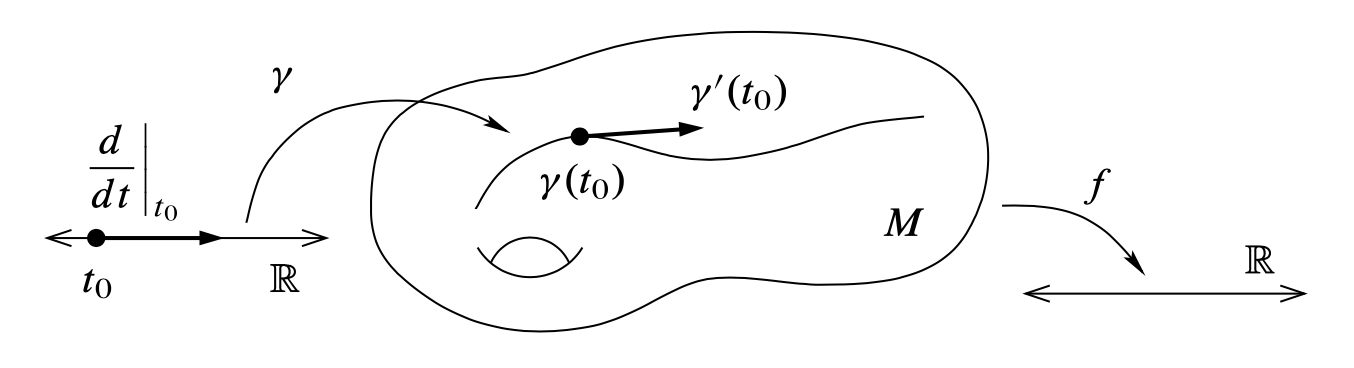
\includegraphics[scale = 0.5]{velocity_of_curve.png}}
\end{minipage}
\caption{\footnotesize{\textbf{The velocity of a curve \citep{lee2003introduction}}}}
\label{fig: velocity_of_curve}
\end{figure}

\item \begin{definition}
Let $M$ be a smooth manifold with or without boundary. Our definition of tangent spaces leads to a natural interpretation of \emph{velocity vectors}: given a smooth curve $\gamma: J \rightarrow M$ and $t_{0} \in J$, we define the \textbf{\emph{velocity of $\gamma$ at $t_0$}} (Fig. \ref{fig: velocity_of_curve}), denoted by $\gamma'(t_0)$, to be the vector
\begin{align*}
\gamma'(t_0) &= d\gamma\paren{\frac{d}{dt}\Bigr|_{t_0}} \in T_{\gamma(t_))}M
\end{align*} where $\frac{d}{dt}\big|_{t_0}$ is the standard coordinate basis vector in $T_{t_0}\bR$. 
\end{definition}

Other common notations for the velocity are
\begin{align*}
\dot{\gamma}(t_0), \quad \frac{d\gamma}{dt}(t_0), \quad \frac{d\gamma}{dt}\Bigr|_{t_0}
\end{align*}

\item \begin{remark}
This tangent vector \emph{\textbf{acts}} on functions by
\begin{align*}
\gamma'(t_0)(f) &= d\gamma\paren{\frac{d}{dt}\Bigr|_{t_0}}(f) = \frac{d}{dt}\Bigr|_{t_0}\paren{f \circ \gamma} = (f \circ \gamma)'(t_0).
\end{align*}
In other words, $\gamma'(t_0)$ is the \emph{\textbf{derivation}} at $\gamma(t_0)$ obtained by taking the \emph{derivative of a function along} $\gamma$. 

If $t_0$ is an endpoint of $J$, this still holds, provided that we interpret the derivative with respect to $t$ as a \emph{one-sided derivative},  or equivalently as the derivative of any smooth extension of $f \circ \gamma$ to an open subset of $\bR$.
\end{remark}

\item \begin{remark}
Now let $(U, \varphi)$ be a smooth chart with coordinate functions $(x^i)$. If $\gamma(t_0) \in U$, we can write the \emph{\textbf{coordinate representation}} of $\gamma$ as $\gamma(t) = (\gamma^1(t), \ldots, \gamma^{n}(t))$, at least for $t$ sufficiently close to $t_0$, and then the \textbf{\emph{coordinate formula}} for the differential yields
\begin{align}
\gamma'(t_0) := d\gamma\paren{\frac{d}{dt}\Bigr|_{t_0}} &= \frac{d\gamma^{i}}{dt}(t_0)\partdiff{}{x^{i}}\Bigr|_{\gamma(t_0)} \label{eqn: curve_coordinate}
\end{align} This means that $\gamma'(t_0)$ is given by essentially the same formula as it would be in \emph{Euclidean space}: it is the tangent vector whose components in a coordinate basis are the derivatives of the component functions of $\gamma$.
\end{remark}

\item The next proposition shows that \emph{every tangent vector on a manifold is the velocity vector of some curve}. This gives a different and somewhat more \emph{\textbf{geometric}} way to think about the \emph{\textbf{tangent bundle}}: it is just \emph{\textbf{the set of all velocity vectors of smooth curves in $M$}}.

\begin{proposition}
Suppose $M$ is a smooth manifold with or without boundary and $p \in M$. Every $v \in T_{p}M$ is the \textbf{velocity} of some smooth curve in $M$.
\end{proposition}

\item \begin{proposition} (\textbf{The Velocity of a Composite Curve}) \citep{lee2003introduction}\\
 Let $F: M \rightarrow N$ be a smooth map, and let $\gamma: J \rightarrow M$ be a smooth curve. For any $t_0 \in J$, the velocity at $t = t_0$ of the composite curve $F \circ \gamma: J \rightarrow N$ is given by
\begin{align}
(F\circ \gamma)'(t_0) &= dF\paren{\gamma'(t_0)}. \label{eqn: curve_composite}
\end{align}
\end{proposition}
Note that
\begin{align*}
(F\circ \gamma)'(t_0) &= d(F\circ \gamma)\paren{\frac{d}{dt}\Bigr|_{t_0}} = dF \circ d\gamma\paren{\frac{d}{dt}\Bigr|_{t_0}} =dF(\gamma'(t_0)). 
\end{align*}

\item \begin{corollary} (\textbf{Computing the Differential Using a Velocity Vector}) \citep{lee2003introduction} \\
Suppose $F: M \rightarrow N$ is a smooth map, $p \in M$, and $v \in T_{p}M$. Then
\begin{align}
dF_{p}(v) = (F \circ \gamma)'(0) \label{eqn: differential_via_curve}
\end{align} for any smooth curve $\gamma: J \rightarrow M$ such that $0 \in J$, $\gamma(0) = p$, and $\gamma'(0) = v$.
\end{corollary} This corollary frequently yields a much more succinct computation of $dF$, especially if $F$ is presented in some form other than an explicit coordinate representation. We will see many examples of this technique in later chapters.
\end{itemize}

\section{Alternative Definitions of the Tangent Space}
In the literature you will find tangent vectors to a smooth manifold defined in several different ways. Here we describe the most common ones.

\begin{remark}
The definition we have chosen, however abstract it may seem at first, has several \textbf{advantages}  \citep{lee2003introduction}:
\begin{itemize}
\item it is relatively \emph{\textbf{concrete}}, i.e. tangent vectors are \textbf{actual derivations} of $\cC^{\infty}(M)$, with \emph{\textbf{no equivalence classes}} involved;
\item it makes the \emph{\textbf{vector space structure}} on $T_{p}M$ obvious; and
\item it leads to straightforward \emph{\textbf{coordinate-independent definitions}} of \emph{differentials}, \emph{velocities}, and many of the other \emph{geometric objects} we will be studying.
\end{itemize}
\end{remark}

\subsection{Tangent Vectors as Derivations of the Space of Germs}
\begin{itemize}
\item \begin{definition}
A \emph{\textbf{smooth function element}} on $M$ is an ordered pair $(f, U)$, where $U$ is an open subset of $M$ and $f: U \rightarrow \bR$ is a smooth function.
\end{definition}

\item \begin{definition}
Given a point $p \in M$, let us define an \textbf{\emph{equivalence relation}} on \emph{the set of all smooth function elements whose domains contain $p$} by setting $(f, U) \sim (g, V)$ if $f \equiv g$ on some neighborhood of $p$.

The \textbf{\emph{equivalence class}} of a function element $(f, U)$ is called \textbf{\emph{the germ of $f$ at $p$}}.
\end{definition}

\item \begin{definition}
The set of \emph{\textbf{all germs of smooth functions}} at $p$ is denoted by $\cC_{p}^{\infty}(M)$. It is a \emph{real vector space} and an \emph{\textbf{associative algebra}} under the operations
\begin{enumerate}
\item $c\brac{(f, U)} = \brac{(cf, U)}$,
\item $\brac{(f, U)} + \brac{(g, V)} = \brac{(f+g, U\cap V)}$
\item $\brac{(f, U)}\brac{(g, V)} = \brac{(f\,g, U\cap V)}$
\end{enumerate}
The \emph{zero element} of this algebra is the equivalence class of the \emph{zero function} on $M$.
\end{definition}

Let us denote the germ at $p$ of the function element $(f, U)$ simply by $[f]_p$. To say that two germs $[f]_{p}$ and $[g]_p$ are equal is simply to say that $f \equiv g$ on some neighborhood of $p$, however small. 

\item \begin{definition}
A \emph{\textbf{derivation}} of $\cC_{p}^{\infty}(M)$ is a \emph{linear map} $v: \cC_{p}^{\infty}(M) \rightarrow \bR$ satisfying the following product product rule:
\begin{align*}
v[f\,g]_{p} &= f(p)\,v[g]_{p} + g(p)\,v[f]_{p}
\end{align*}
\end{definition}

\item It is common to define the \emph{\textbf{tangent space}} to $M$ at $p$ as the vector space $\mathfrak{D}_{p}M$ of derivations of $\cC_{p}^{\infty}(M)$. 

\item The germ definition has a number of \textbf{advantages}. One of the most significant is that it makes the \emph{\textbf{local nature}} of the \emph{tangent space} clearer, without requiring the use of \textbf{\emph{bump functions}} (i.e. $\varphi$). Because there do not exist \emph{analytic bump functions}, the germ definition of tangent vectors is the only one available on \emph{real-analytic} or \emph{complex-analytic manifolds}. 

\item The chief \textbf{disadvantage} of the germ approach is simply that it adds an additional level of \textbf{complication} to an already highly abstract definition.
\end{itemize}
\subsection{Tangent Vectors as Equivalence Classes of Curves}
\begin{itemize}
\item Another common approach to tangent vectors is to define an \emph{\textbf{intrinsic equivalence relation}} on the set of \textbf{smooth curves} with the same starting point, which captures the idea of "\emph{having the same velocity,}" and to define a \emph{tangent vector} as \emph{an equivalence class of curves}. Here we describe one such equivalence relation.

\item \begin{definition}
Suppose $p$ is a point of $M$. We wish to define an \textbf{equivalence relation} on the set of \emph{all smooth curves of the form} $\gamma: J \rightarrow M$, where $J$ is an interval containing $0$ and $\gamma(0) = p$. 

Given two such curves $\gamma_1: J_1 \rightarrow M$ and $\gamma_2: J_2 \rightarrow M$, let us say that $\gamma_1 \sim \gamma_2$ if $(f \circ \gamma_1)'(0) = (f \circ \gamma_2)'(0)$ for \emph{\textbf{every smooth real-valued function}} $f$ defined in a neighborhood of $p$. 

Let $\cV_{p}M$ denote the \emph{\textbf{set of equivalence classes}}. The \emph{\textbf{tangent space}} to $M$ at $p$ is often defined to be the set $\cV_{p}M$.
\end{definition}

\item \begin{definition}
Define the \emph{\textbf{differential}} of a smooth map $F: M \rightarrow N$ as the map that sends $[\gamma] \in \cV_{p}M$ to $[F\circ \gamma] \in \cV_{F(p)}N$. 
\end{definition}

\item  Velocity vectors of smooth curves are almost as easy to define. 
\begin{definition}
Suppose $\gamma: J \rightarrow M$ is any smooth curve. If $0 \in J$, then \emph{the \textbf{velocity} of $\gamma$ at $0$} is just \emph{\textbf{the equivalence class}} of $\gamma$ in $\cV_{\gamma(0)}M$. 

The velocity at any other point $t_0 \in J$ can be defined as the equivalence class in $\cV_{\gamma(t_0)}M$ of the curve $\gamma(t_0)$ defined by $\gamma(t_0)(t) =  \gamma(t_0 + t)$. 
\end{definition}

\end{itemize}
\subsection{Tangent Vectors as Equivalence Classes of $n$-Tuples}
\begin{itemize}
\item Yet another approach to defining the tangent space is based on the transformation rule \eqref{eqn: tangent_vec_decomp} for the components of tangent vectors in coordinates.
\begin{align*}
v&=v^{i} \partdiff{}{x^{i}}\Bigr|_{p} 
\end{align*}

\item One defines a \emph{\textbf{tangent vector}} at a point $p \in M$ to be a rule that assigns an ordered $n$-tuple $(v^1,\ldots, v^n) \in \bR^n$ to \emph{\textbf{each smooth coordinate chart containing}} $p$, with the property that the $n$-tuples assigned to overlapping charts transform according to \eqref{eqn: tangent_vec_decomp}. (This is, in fact, the oldest definition of all, and many physicists are still apt to think of tangent vectors this way.)

\item In this approach, the \emph{\textbf{velocity of a curve}} is defined by the usual \emph{Euclidean formula} in coordinates, and the \emph{\textbf{differential}} of $F: M \rightarrow N$ is defined as the \emph{linear map} determined by the \textbf{Jacobian matrix} of $F$ \emph{\textbf{in coordinates}}. One then has to \textbf{show}, by means of \emph{tedious computations} involving the chain rule, that these operations are well defined, \emph{\textbf{independently of the choices of coordinates}}.
\end{itemize}
\newpage
\bibliographystyle{plainnat}
\bibliography{book_reference.bib}
\end{document}